\clearpage
\section{Top-hat Function Analysis}
We want to analyze the top-hat function and how its Fourier transform behaves in the reciprocal domain.
% The following is the top-hat function that we are using in our methodology:
% \begin{flalign}
%     \phi(z) &= \frac{1}{1+ exp(-\gamma(0.5L+z))} + \frac{1}{1+ exp(-\gamma(0.5L-z))} -1
% \end{flalign}
% This function uses a linear combination of two sigmoid functions to make a symmetrical top-hat function about the origin. The constant \textbf{$\gamma$} determines the steepness of the top-hat around the edges. 
% Other forms of the top-hat functions can also be used; some examples are as follows:
% \begin{flalign*}
%         \phi(z) &= \frac{1}{2}[ \tanh(\gamma(x + 0.5L)) -\tanh(\gamma(x - 0.5L)) ] \\
%         \phi(z) &= \frac{2}{\pi}\left[ \arctan \left( e^{\gamma (-x + 0.5L)} \right) + \arctan \left( e^{\gamma (x + 0.5L)} \right) \right]- 1 
% \end{flalign*}
% The behaviour of this function (1) is as follows:

\subsection*{Background}
In our modified approach to the 2D Ewald summation, we have incorporated a top-hat function and performed a Fourier integral of this function. It is well understood that the Fourier transform of a top-hat function produces an oscillatory output. We hypothesize that these oscillations contribute to the instability of our method, thereby impeding our goal of achieving lower error rates. Therefore, our current objective is to refine the top-hat function to minimize oscillatory behaviour.
\subsubsection*{Equations}
In the final form of the reciprocal energy, we have the following expression,
\begin{flalign*}
    (4\pi\epsilon_o)U^{LR}& =\frac{\sqrt{\pi}}{L_xL_y}\sum_{\vec K=-\infty}^{\infty}\prime\left[ \int_{0}^{\alpha}\frac{dt}{t^2}C_{k_z}(t)\textrm{ exp}\left(\frac{-1}{4t^2}|\vec G|_{xy}^2\right)\right] |\,S(\vec G)\,|^2
\end{flalign*}
In the equation presented above, the term enclosed within the square brackets is independent of the specific configuration of the simulation cell, i.e. it does not depend on the spatial distribution or positions of the ions, but only depends on the cell's side lengths. The term $C_{k_z}(t)$ is expressed as follows:
\begin{flalign*}
     C_{k_z}(t) &=\frac{1}{L_z}\int_{-\infty}^{\infty}ds\hspace{1mm}exp(-i\frac{2\pi n s}{L_z})\hspace{1mm} exp(-s^2t^2)\, \phi(s) 
     % \\ &=\frac{1}{L_z}\int_{-\infty}^{\infty}ds\hspace{1mm}exp(-i\frac{2\pi n s}{L_z})\hspace{1mm} exp(-s^2t^2)\left[\frac{1}{1+ exp(-\gamma(0.5L_z+s))} + \frac{1}{1+ exp(-\gamma(0.5L_z-s))} -1\right]
\end{flalign*}
We can observe that the above term is a fourier transform of the product of a top-hat $\phi (s)$ and a gaussian function. We hypothesize that most of the oscillations in our calculations are due to the top-hat function. We want to observe the behaviour of its fourier transform by varying its parameters ($\gamma$ \& $L_z$).

\subsection*{Analysis}

In Fig.~\ref{fig:tophat}, as $\gamma$ decreases, the top-hat function becomes more localized and narrower in real space, while larger values of $\gamma$ result in a broader profile. However, broader top-hat functions lead to widespread and sustained oscillations in the frequency domain (Fig.~\ref{fig:fourieroftophatvarygammaL300}), which can negatively impact the convergence of numerical computations for reciprocal space energies. To reduce these oscillations, we prefer using smaller values of $\gamma$, which yield narrower functions in real space and faster-decaying Fourier transforms. The downside of using smaller $\gamma$ is that it reduces the region where the top-hat function remains exactly one. We must increase the domain length $L_z$ to ensure the simulation box lies entirely within this region.

\begin{figure}[htbp]
  \centering
  \begin{minipage}[b]{0.45\textwidth}
    \centering
    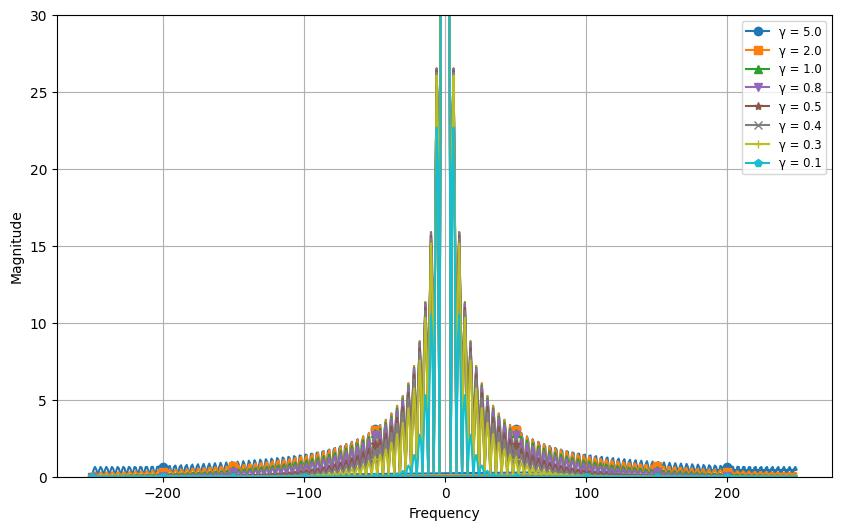
\includegraphics[width=\linewidth]{images/fourieroftophatvarygammaL300.jpg}
    \caption{Fourier Transform of Top-hat Function with Varying $\gamma$, $L_z = 300$}
    \label{fig:fourieroftophatvarygammaL300}
  \end{minipage}
  \hfill
  \begin{minipage}[b]{0.45\textwidth}
    \centering
    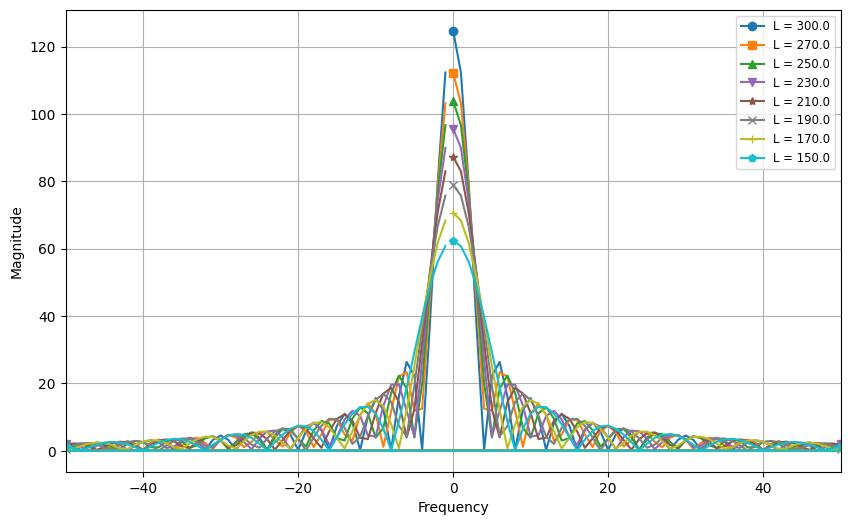
\includegraphics[width=\linewidth]{images/fourieroftophatvaryL_gamma0.5.jpg}
    \caption{Fourier Transform of Top-hat Function with Varying $L_z$, $\gamma = 0.5$}
    \label{fig:fourieroftophatvaryL_gamma0}
  \end{minipage}
\end{figure}

Fig.~\ref{fig:fourieroftophatvaryL_gamma0} supports this choice by showing the Fourier Transform for varying $L_z$ at a fixed $\gamma = 0.5$. It demonstrates that changing $L_z$ does not impact the convergence or magnitude of the oscillations in the frequency domain. Although the damping frequency, where oscillations begin to decay, shifts higher with larger $L_z$, this does not affect the essential behaviour of the transform. This confirms that increasing $L_z$ when using smaller $\gamma$ values does not introduce computational issues, making this a suitable strategy for reducing oscillations while preserving accuracy.

\subsubsection*{Choosing $L_z$}
The motivation for introducing the top-hat function was to strictly enforce the condition:
\begin{flalign*}
\phi(z) = \begin{cases} 
        1 & \text{if } z \in (-\frac{L_z}{2}, \frac{L_z}{2}) \\
        0 & \text{otherwise}
\end{cases}
\end{flalign*}
In our implementation, we use a continuous version of $\phi(z)$, which transitions over a finite region rather than switching sharply between 0 and 1. To ensure the simulation cell lies fully within the region where $\phi(z) = 1 $, we choose the smallest possible $L_z$. This also helps reduce the number of grid points required in the SPME (Smooth Particle Mesh Ewald) method, thereby improving computational efficiency. To find the optimal $L_z$ we implemented the binary search based algorithm (\textbf{Alg. \ref{alg:vacuum}}), to find the required box length.

\begin{algorithm}[H]
\caption{Binary Search to Find Simulation Box Vacuum}
\label{alg:vacuum}
\KwData{Side Length: $L > 0$, gamma: $\gamma$}
\KwResult{Optimum vacuum for simulation box}
\textbf{Input:} Side Length: $L$, gamma: $\gamma$, \textbf{Optional: }margin = 5, maxVacuum = 1000 \\
$\text{low} \gets 2 \times L$,
$\text{high} \gets \text{maxVacuum}$

\While{$\text{high} - \text{low} > 1$}{
    $\text{mid} \gets \frac{\text{low} + \text{high}}{2}$ \;
    \If{$\text{tophat}(L, \gamma, \text{mid}) == 1$}{
        $\text{high} \gets \text{mid}$ \;
    }
    \Else{
        $\text{low} \gets \text{mid}$ \;
    }
}
\Return $\text{margin} + \text{high} $\;
\end{algorithm}
